% Options for packages loaded elsewhere
\PassOptionsToPackage{unicode}{hyperref}
\PassOptionsToPackage{hyphens}{url}
%
\documentclass[
]{article}
\usepackage{amsmath,amssymb}
\usepackage{iftex}
\ifPDFTeX
  \usepackage[T1]{fontenc}
  \usepackage[utf8]{inputenc}
  \usepackage{textcomp} % provide euro and other symbols
\else % if luatex or xetex
  \usepackage{unicode-math} % this also loads fontspec
  \defaultfontfeatures{Scale=MatchLowercase}
  \defaultfontfeatures[\rmfamily]{Ligatures=TeX,Scale=1}
\fi
\usepackage{lmodern}
\ifPDFTeX\else
  % xetex/luatex font selection
\fi
% Use upquote if available, for straight quotes in verbatim environments
\IfFileExists{upquote.sty}{\usepackage{upquote}}{}
\IfFileExists{microtype.sty}{% use microtype if available
  \usepackage[]{microtype}
  \UseMicrotypeSet[protrusion]{basicmath} % disable protrusion for tt fonts
}{}
\makeatletter
\@ifundefined{KOMAClassName}{% if non-KOMA class
  \IfFileExists{parskip.sty}{%
    \usepackage{parskip}
  }{% else
    \setlength{\parindent}{0pt}
    \setlength{\parskip}{6pt plus 2pt minus 1pt}}
}{% if KOMA class
  \KOMAoptions{parskip=half}}
\makeatother
\usepackage{xcolor}
\usepackage{graphicx}
\usepackage{subcaption}
\makeatletter
\def\maxwidth{\ifdim\Gin@nat@width>\linewidth\linewidth\else\Gin@nat@width\fi}
\def\maxheight{\ifdim\Gin@nat@height>\textheight\textheight\else\Gin@nat@height\fi}
\makeatother
% Scale images if necessary, so that they will not overflow the page
% margins by default, and it is still possible to overwrite the defaults
% using explicit options in \includegraphics[width, height, ...]{}
\setkeys{Gin}{width=\maxwidth,height=\maxheight,keepaspectratio}
% Set default figure placement to htbp
\makeatletter
\def\fps@figure{htbp}
\makeatother
\setlength{\emergencystretch}{3em} % prevent overfull lines
\providecommand{\tightlist}{%
  \setlength{\itemsep}{0pt}\setlength{\parskip}{0pt}}
\setcounter{secnumdepth}{-\maxdimen} % remove section numbering
\ifLuaTeX
  \usepackage{selnolig}  % disable illegal ligatures
\fi
\IfFileExists{bookmark.sty}{\usepackage{bookmark}}{\usepackage{hyperref}}
\IfFileExists{xurl.sty}{\usepackage{xurl}}{} % add URL line breaks if available
\urlstyle{same}
\hypersetup{
  pdftitle={Alberi binari di ricerca e alberi rosso-neri},
  pdfauthor={Leonardo Toccafondi},
  hidelinks,
  pdfcreator={LaTeX via pandoc}}

\title{Alberi binari di ricerca e alberi rosso-neri}
\author{Leonardo Toccafondi}
\date{February 2023}

\begin{document}
\maketitle

\hypertarget{introduzione}{%
\section{Introduzione}\label{introduzione}}

In questa relazione si andranno a confrontare alberi binari di ricerca e
alberi rosso-neri, al fine di determinare le differenze, e di
conseguenza i loro vantaggi e svantaggi, tra queste due strutture dati.

\hypertarget{descrizione-teorica-delle-strutture-dati}{%
\section{Descrizione teorica delle strutture
dati}\label{descrizione-teorica-delle-strutture-dati}}

Un albero è una struttura dati composta da elementi, detti nodi: ognuno
contiene una chiave che lo identifica univocamente. Inoltre, può
contenere anche altri campi, come ad esempio un puntatore ai nodi
\emph{figli}. Il nodo dal quale discendono tutti gli altri nodi viene
detto \emph{radice} (in inglese root). Un nodo che non possiede figli è
detto \emph{foglia}. Viene definito \emph{cammino} da un nodo un nodo n
ad un nodo m una sequenza di nodi connessi da archi che portano da n ad
m. La \emph{lunghezza del cammino} è pari al numero di nodi che si
incontrano nel cammino, escluso il primo. Di conseguenza la lunghezza di
un cammino contenente un solo nodo è pari a 0. Si dice \emph{altezza}
\(h\) dell'albero la lunghezza massima tra i cammini che uniscono la
radice alla foglie. Un albero binario è un albero in cui ogni nodo ha
\emph{al massimo} due figli.

\hypertarget{albero-binario-di-ricerca}{%
\subsubsection{Albero binario di
ricerca}\label{albero-binario-di-ricerca}}

Si considera un albero binario di ricerca (abbreviato ABR o BST da
binary search tree) come un albero binario ogni nodo è un oggetto con i
campi key, left, right, p (rispettivamente la chiave, il puntatore al
figlio sinistro, il puntatore al figlio destro e un puntatore al padre).
I nodi dei un albero binario devono rispettare una proprietà: sia x un
nodo e y un nodo del sottoalbero sinistro di x, allora
\(y.key \leq x.key\) . Viceversa se y è un nodo del sotto albero
\emph{destro} di x.

Il bilanciamento di un ABR dipende dall'ordine di inserimento dei nodi:
nel caso di un inserimento ordinato (sia crescente che decrescente),
l'albero sarà sbilanciato rispettivamente tutto a destra o tutto a
sinistra. L'albero è perfettamente bilanciato quando ogni nodo, escluse
le foglie, ha esattamente due figli.

\hypertarget{albero-rosso-nero}{%
\subsubsection{Albero rosso-nero}\label{albero-rosso-nero}}

Un albero rosso-nero (abbreviato ARN o RBT da red-black tree) è un ABR
dove ogni nodo possiede anche un parametro per il colore. Quest'ultimo è
un attributo booleano (x.colour) e può essere \emph{rosso} o
\emph{nero}. Eredita tutti gli attributi di un ABR. In un ARN esistono
le \emph{foglie vuote} o \emph{NIL}. Tra quest'ultime e le foglie nere
vi è una relazione:

\begin{itemize}
\item
  ad ogni foglia di T è posta una sentinella T.nil
\item
  il colore della foglia vuota è nero
\item
  La foglia vuota è padre della radice
\item
  Non interessa la chiave della foglia vuota~
\end{itemize}

\hypertarget{proprietuxe0}{%
\paragraph{Proprietà}\label{proprietuxe0}}

In un albero rosso-nero sono soddisfatte le seguenti proprietà:

\begin{itemize}
\item
  Ogni nodo è rosso o nero
\item
  La radice è nera
\item
  Ogni foglia (T.nil) è nera
\item
  Se un nodo è rosso, allora entrambi i suoi figli sono neri
\item
  Tutti i cammini da ogni nodo alle sue foglie contengono lo stesso
  numero di nodi neri
\end{itemize}

Gli ARN garantiscono la non-esistenza di un qualsiasi cammino dalla
radice ad una foglia qualsiasi che sia lungo più del doppio di qualsiasi
altro. Ciò, insieme all'ultima proprietà che fa in modo che i nodi neri
siano distribuiti nello stesso modo in tutti i cammini, rendono un ARN
\emph{bilanciato.} Per un nodo di un albero rosso-nero è possibile
definire due tipi di altezze: \(h(x)\), che rappresenta l'altezza del
nodo x, ovvero il numero di archi nel cammino più lungo fino ad una
foglia; \(bh(x)\) o \emph{altezza nera}, pari al numero dei nodi neri
(inclusa T.nil ed escluso x) nel cammino da x alla foglia. Queste
servono a definire l'altezza di un albero rosso-nero con n nodi interni
(ovvero con almeno una foglia): \(h \leq 2 \lg(n+1)\)

\hypertarget{teoria-a-base-degli-esperimenti}{%
\section{Teoria a base degli
esperimenti}\label{teoria-a-base-degli-esperimenti}}

Le operazioni che non vanno a modificare l'albero, come ad esempio la
ricerca di un nodo sia per l'ABR che per l'ARN impiegano un tempo pari
ad \({O}(h)\), quindi hanno un costo proporzionale all'altezza
dell'albero stesso.

Nel caso peggiore per un albero binario di ricerca (che ricordiamo
avvenire nel caso di un inserimento in ordine, con conseguente
sbilanciamento dell'albero) abbiamo che l'altezza \(h\) è pari al numero
di nodi n - 1. Quindi tutte e tre le operazioni, nel caso peggiore per
gli alberi binari di ricerca, necessitano di un tempo pari a \({O}(n)\).
Per alcune permutazioni dell'ordine degli inserimenti, l'albero risulta
perfettamente bilanciato e \(h = {O}(lg(n))\). L'altezza è proporzionale
al logaritmo del numero di nodi: ciò a grandi linee vale anche per gli
inserimenti randomici, anche se con delle costanti di tempo maggiori.

Per quanto riguarda gli alberi rosso-neri, grazie alle loro proprietà
riguardanti l'altezza, nel caso peggiore gli algoritmi impiegano un
tempo pari a \({O}(lg(n))\). Nel caso medio

Dal momento che \({O}(h)\) è il costo di un singolo inserimento di un
nodo, il costo di \(n\) inserimenti sarà pari a \({O}(n*h)\),

\hypertarget{descrizione-ed-implementazione-degli-esperimenti}{%
\section{Descrizione ed implementazione degli
esperimenti}\label{descrizione-ed-implementazione-degli-esperimenti}}

Per confrontare queste due strutture dati, eseguiremo dei semplici test
su due operazioni comuni: inserimento e ricerca di nodi. Inoltre,
valuteremo anche l'altezza degli alberi risultanti. Tutto questo sarà
valutato all'aumentare del numero di nodi n, partendo da 100 fino ad
arrivare a 10000. I test saranno effettuati ogni 100 nodi aggiuntivi.
Inoltre, per il caso randomizzato, verrà effettuato un'ulteriore test,
dove il numero massimo di nodi sarà 100000, con test effettuati ogni
1000 inserimenti di nodo.

Confronteremo gli ABR e gli ARN in base all'ordine in cui sono inseriti
i nodi, considerando il ``caso peggiore'', ovvero con l'inserimento
ordinato per determinare quanto più sia bilanciato l'albero rosso-nero
rispetto all'albero binario di ricerca. Oltre a ciò valuteremo quello
che per gli alberi rosso-neri è il caso medio: con un inserimento dello
stesso vettore di nodi del caso peggiore, ma randomizzato per
avvicinarci il più possibile al caso migliore per entrambi, anche se nel
caso dell'albero binario di ricerca non abbiamo un albero completo. Per
quanto riguarda la ricerca, in entrambi i test viene generato un numero
pseudorandomico compreso tra 1 e il numero di nodi della permutazione
presa in considerazione, e ne viene effettuata la ricerca all'interno
dell'albero.

\hypertarget{implementazione-python}{%
\paragraph{Implementazione python}\label{implementazione-python}}

\

Il programma che esegue il test è composto da 3 file python:

\begin{itemize}
\tightlist
\item
  BST.py: contiene l'implementazione dell'albero binario di ricerca.  All'interno del file si trova una classe Node, che rappresenta un nodo
  dell'ABR e che quindi contiene tutti i campi necessari; ed una classe  BST, (caratterizzata da un solo attributo root) che implementa le
  funzioni di inserimento, cancellazione, altezza e \emph{trapianto}
  dell'albero binario di ricerca.
\item
  RBT.py: contiene l'implementazione dell'albero rosso-nero. Il file
  contiene sia una classe Node, che rapprensenta un nodo dell'ARN
  (quindi non solo la chiave, il nodo padre e i figli, ma anche il
  \emph{colore}), mentre invece la classe RBT implementa un albero
  rosso-nero con tutte le sue funzioni: inserimento, ricerca di un nodo,
  rotazioni e \emph{``fixup''} del colore.
\item
  test.py: si occupa dello svolgimento dell'esperimento (utilizzando
  matplotlib, numpy) e della creazione dei grafici necessari alla
  visualizzazione dei risultati. Viene inoltre calcolata la \emph{media
  mobile cumulativa} ad ogni misurazione. Ciò viene fatto, insieme ad un
  calcolo di una b-spline prima del plotting, al fine di \emph{smussare}
  i grafici.
\end{itemize}

\hypertarget{ambiente-di-test}{%
\paragraph{Ambiente di test}\label{ambiente-di-test}}
\

L'esperimento è stato svolto su un computer con le seguenti
caratteristiche:

\begin{itemize}
\item
  Sistema operativo: Linux Mint 21.1 con kernel 5.15
\item
  CPU: Inter Core i7-9750H
\item
  RAM: 16 GB
\item
  Interprete Python: conda 22.11.1 e python v 3.10
\item
  IDE: Pycharm Community Edition 2022.3.2
\end{itemize}

\hypertarget{risultati-dellesperimento}{%
\section{Risultati dell'esperimento}\label{risultati-dellesperimento}}

\hypertarget{inserimento}{%
\subsubsection{Inserimento}\label{inserimento}}


\begin{figure}[h!]
	\centering
	\begin{subfigure}[b]{0.4\linewidth}
		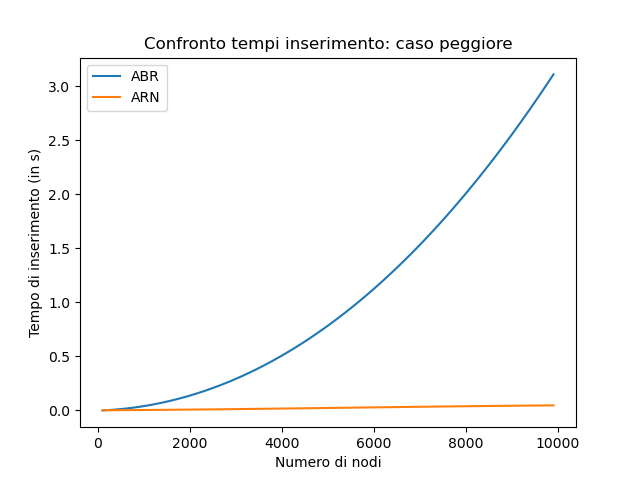
\includegraphics[width=\linewidth]{../../img/w_case/ins_10000.png}
	\end{subfigure}
	\begin{subfigure}[b]{0.4\linewidth}
		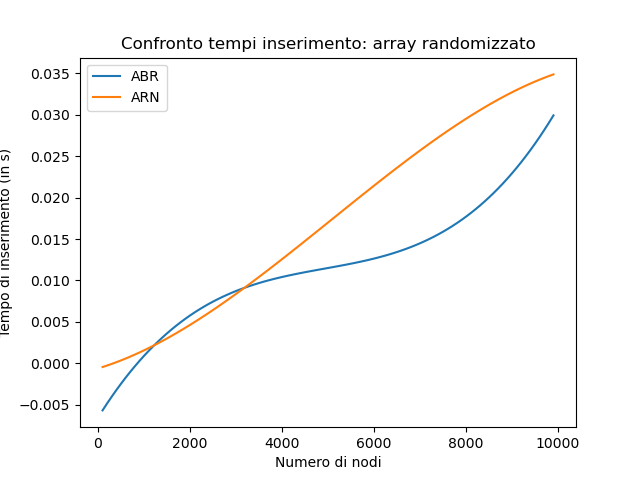
\includegraphics[width=\linewidth]{../../img/rand/ins_10000.png}
	\end{subfigure}
	\caption{Tempo di inserimento 10000 nodi}
	\label{fig:1}
\end{figure}


\begin{figure}[h!]
	\centering
	\begin{subfigure}[b]{0.4\linewidth}
		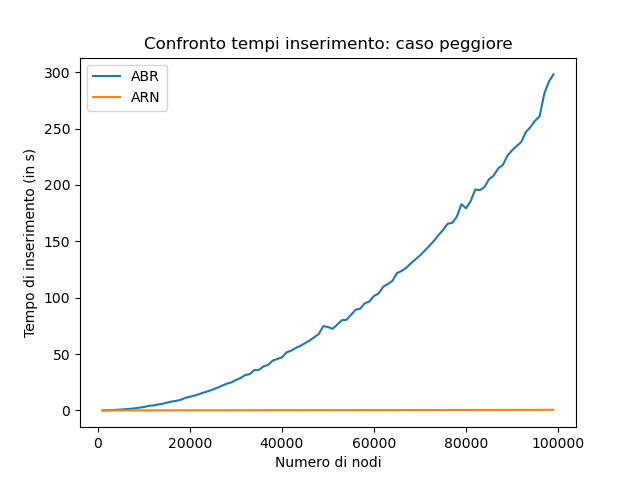
\includegraphics[width=\linewidth]{../../img/w_case/ins_100000.png}
	\end{subfigure}
	\begin{subfigure}[b]{0.4\linewidth}
		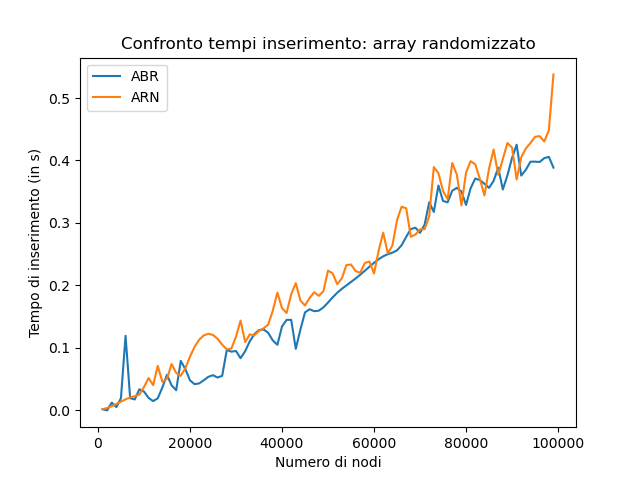
\includegraphics[width=\linewidth]{../../img/rand/ins_100000.png}
	\end{subfigure}
	\caption{Tempo di inserimento 100000 nodi}
	\label{fig:2}
\end{figure}

\newpage
\hypertarget{ricerca}{%
\subsubsection{Ricerca}\label{ricerca}}


\begin{figure}[h!]
	\centering
	\begin{subfigure}[b]{0.4\linewidth}
		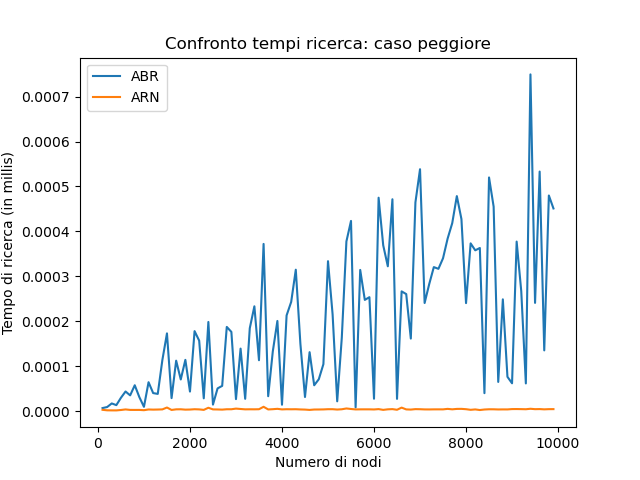
\includegraphics[width=\linewidth]{../../img/w_case/s_10000.png}
	\end{subfigure}
	\begin{subfigure}[b]{0.4\linewidth}
		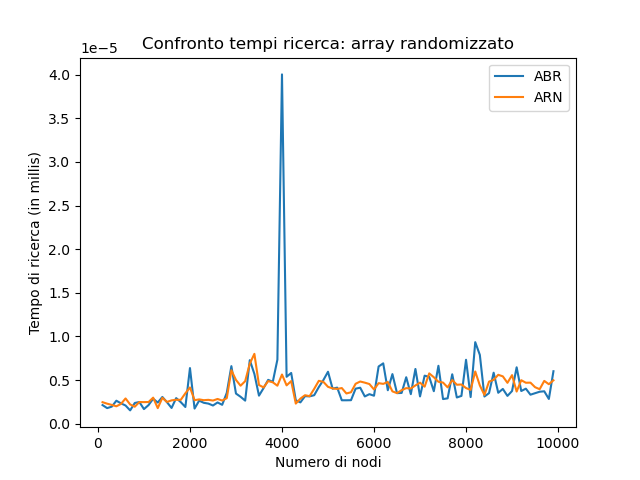
\includegraphics[width=\linewidth]{../../img/rand/s_10000.png}
	\end{subfigure}
	\caption{Tempo di ricerca 10000 nodi}
	\label{fig:3}
\end{figure}


\begin{figure}[h!]
	\centering
	\begin{subfigure}[b]{0.4\linewidth}
		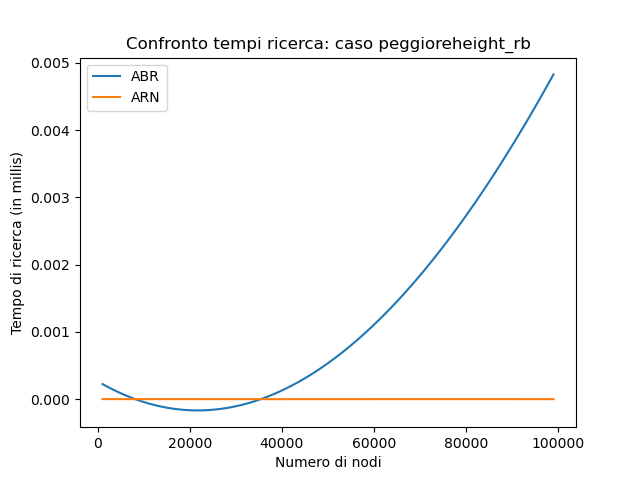
\includegraphics[width=\linewidth]{../../img/w_case/s_100000.png}
	\end{subfigure}
	\begin{subfigure}[b]{0.4\linewidth}
		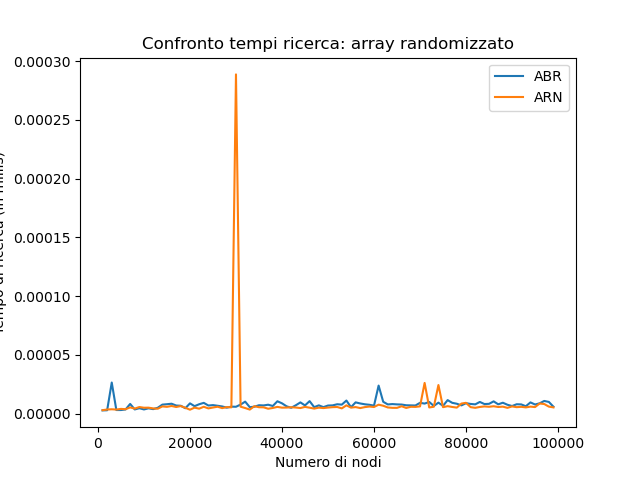
\includegraphics[width=\linewidth]{../../img/rand/s_100000.png}
	\end{subfigure}
	\caption{Tempo di ricerca 100000 nodi}
	\label{fig:4}
\end{figure}

\hypertarget{altezza}{%
\subsubsection{Altezza}\label{altezza}}

\begin{figure}[h!]
	\centering
	\begin{subfigure}[b]{0.4\linewidth}
		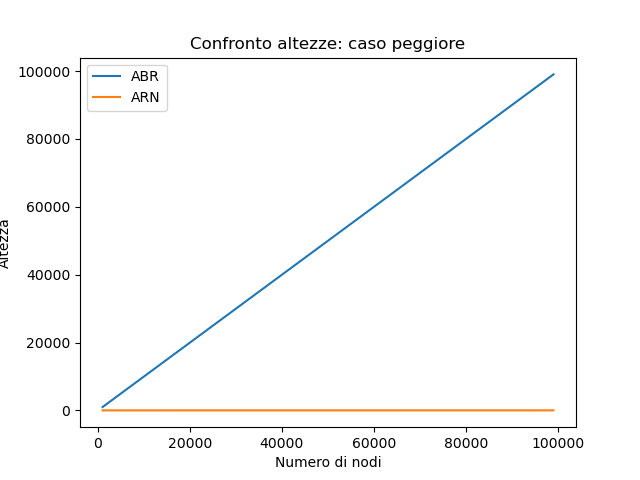
\includegraphics[width=\linewidth]{../../img/w_case/h_100000.png}
	\end{subfigure}
	\begin{subfigure}[b]{0.4\linewidth}
		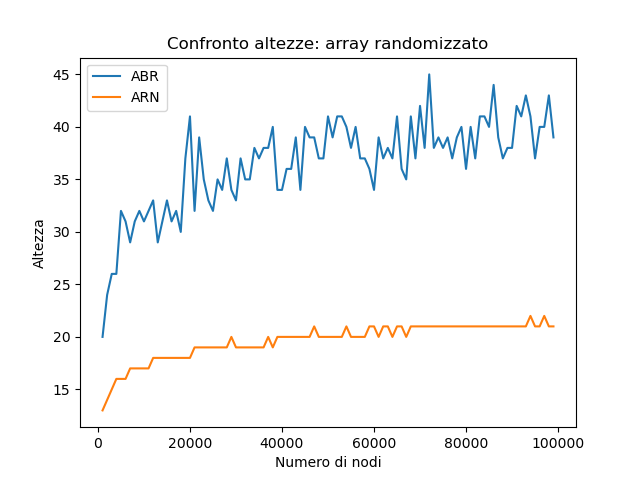
\includegraphics[width=\linewidth]{../../img/rand/h_100000.png}
	\end{subfigure}
	\caption{Confronto altezze: 100000 nodi}
	\label{fig:5}
\end{figure}

\newpage

\hypertarget{commento-e-conclusioni}{%
\section{Commento e conclusioni}\label{commento-e-conclusioni}}

Come possiamo vedere dai grafici, nel caso peggiore l'albero binario di
ricerca ha delle performance peggiori, soprattutto nell'altezza, che da
definizione è pari a \({O}(n)\). Anche per l'inserimento e per la
ricerca gli alberi rosso-neri impiegano un tempo decisamente minore
rispetto agli alberi binari di ricerca.

Passando invece all'inserimento randomizzato, la differenza tra le due
strutture si assottiglia notevolmente, anche nel caso della ricerca,
rispettando la complessità \({O}(logn)\). Per quanto riguarda
l'inserimento, sia per quanto riguarda il caso con 10000 nodi, sia
quello con 100000, gli alberi rosso-neri hanno una performance sempre in
linea con i valori prospettati, ma comunque peggiore (anche se non di
molto) rispetto all'inserimento in un albero binario di ricerca. Si nota
tuttavia un miglioramento importante nelle altezze degli alberi binari
di ricerca, avvicindandosi \emph{notevolmente} a quelle degli alberi
rosso-neri.

In conclusione, risulta preferibile l'implementazione di alberi
rosso-neri, a scapito di una maggiore semplicità di realizzazione degli
ARN.

\end{document}
